
\chapter{Probability density functions}
\label{density}
\index{PDF}
\index{probability density function}
\index{exponential distribution}
\index{distribution!exponential}
\index{normal distribution}
\index{distribution!normal}
\index{Gaussian distribution}
\index{distribution!Gaussian}
\index{CDF}
\index{derivative}

The code for this chapter is in {\tt density.py}.  For information
about downloading and working with this code, see Section~\ref{code}.


\section{PDFs}

The derivative of a CDF is called a {\bf probability density function},
or PDF.  For example, the PDF of an exponential distribution is
%
\[ \PDF_{expo}(x) = \lambda e^{-\lambda x}   \]
%
The PDF of a normal distribution is
%
\[ \PDF_{normal}(x) = \frac{1}{\sigma \sqrt{2 \pi}} 
                 \exp \left[ -\frac{1}{2} 
                 \left( \frac{x - \mu}{\sigma} \right)^2 \right]  \]
%
Evaluating a PDF for a particular value of $x$ is usually not useful.
The result is not a probability; it is a probability {\em density}.
\index{density}
\index{mass}

In physics, density is mass per unit of
volume; in order to get a mass, you have to multiply by volume or,
if the density is not constant, you have to integrate over volume.

Similarly, {\bf probability density} measures probability per unit of $x$.
In order to get a probability mass, you have to integrate over $x$.

{\tt thinkstats2} provides a class called Pdf that represents
a probability density function.  Every Pdf object provides the
following methods:

\begin{itemize}

\item {\tt Density}, which takes a value, {\tt x}, and returns the
  density of the distribution at {\tt x}.

\item {\tt Render}, which evaluates the density at a discrete set of
  values and returns a pair of sequences: the sorted values, {\tt xs},
  and their probability densities, {\tt ds}.

\item {\tt MakePmf}, which evaluates {\tt Density}
  at a discrete set of values and returns a normalized Pmf that
  approximates the Pdf.
\index{Pmf}

\item {\tt GetLinspace}, which returns the default set of points used 
  by {\tt Render} and {\tt MakePmf}.

\end{itemize}  

Pdf is an abstract parent class, which means you should not
instantiate it; that is, you cannot create a Pdf object.  Instead, you
should define a child class that inherits from Pdf and provides
definitions of {\tt Density} and {\tt GetLinspace}.  Pdf provides
{\tt Render} and {\tt MakePmf}.

For example, {\tt thinkstats2} provides a class named {\tt
  NormalPdf} that evaluates the normal density function.

\begin{verbatim}
class NormalPdf(Pdf):

    def __init__(self, mu=0, sigma=1, label=''):
        self.mu = mu
        self.sigma = sigma
        self.label = label

    def Density(self, xs):
        return scipy.stats.norm.pdf(xs, self.mu, self.sigma)

    def GetLinspace(self):
        low, high = self.mu-3*self.sigma, self.mu+3*self.sigma
        return np.linspace(low, high, 101)
\end{verbatim}

The NormalPdf object contains the parameters {\tt mu} and
{\tt sigma}.  {\tt Density} uses
{\tt scipy.stats.norm}, which is an object that represents a normal
distribution and provides {\tt cdf} and {\tt pdf}, among other
methods (see Section~\ref{normal}).
\index{SciPy}

The following example creates a NormalPdf with the mean and variance
of adult female heights, in cm, from the BRFSS (see
Section~\ref{brfss}).  Then it computes the density of the
distribution at a location one standard deviation from the mean.
\index{standard deviation}

\begin{verbatim}
>>> mean, var = 163, 52.8
>>> std = math.sqrt(var)
>>> pdf = thinkstats2.NormalPdf(mean, std)
>>> pdf.Density(mean + std)
0.0333001
\end{verbatim}

The result is about 0.03, in units of probability mass per cm.
Again, a probability density doesn't mean much by itself.  But if
we plot the Pdf, we can see the shape of the distribution:

\begin{verbatim}
>>> thinkplot.Pdf(pdf, label='normal')
>>> thinkplot.Show()
\end{verbatim}

{\tt thinkplot.Pdf} plots the Pdf as a smooth function,
as contrasted with {\tt thinkplot.Pmf}, which renders a Pmf as a
step function.  Figure~\ref{pdf_example} shows the result, as well
as a PDF estimated from a sample, which we'll compute in the next
section.
\index{thinkplot}

You can use {\tt MakePmf} to approximate the Pdf:

\begin{verbatim}
>>> pmf = pdf.MakePmf()
\end{verbatim}

By default, the resulting Pmf contains 101 points equally spaced from
{\tt mu - 3*sigma} to {\tt mu + 3*sigma}.  Optionally, {\tt MakePmf}
and {\tt Render} can take keyword arguments {\tt low}, {\tt high},
and {\tt n}.

\begin{figure}
% pdf_example.py
\centerline{\includegraphics[height=2.2in]{figs/pdf_example.pdf}}
\caption{A normal PDF that models adult female height in the U.S.,
and the kernel density estimate of a sample with $n=500$.}
\label{pdf_example}
\end{figure}


\section{Kernel density estimation} 

{\bf Kernel density estimation} (KDE) is an algorithm that takes
a sample and finds an appropriately smooth PDF that fits 
the data.  You can read details at
\url{http://en.wikipedia.org/wiki/Kernel_density_estimation}.
\index{KDE}
\index{kernel density estimation}

{\tt scipy} provides an implementation of KDE and {\tt thinkstats2}
provides a class called {\tt EstimatedPdf} that uses it:
\index{SciPy}
\index{NumPy}

\begin{verbatim}
class EstimatedPdf(Pdf):

    def __init__(self, sample):
        self.kde = scipy.stats.gaussian_kde(sample)

    def Density(self, xs):
        return self.kde.evaluate(xs)
\end{verbatim}

\verb"__init__" takes a sample
and computes a kernel density estimate.  The result is a
\verb"gaussian_kde" object that provides an {\tt evaluate}
method.

{\tt Density} takes a value or sequence, calls
\verb"gaussian_kde.evaluate", and returns the resulting density.  The
word ``Gaussian'' appears in the name because it uses a filter based
on a Gaussian distribution to smooth the KDE.  \index{density}

Here's an example that generates a sample from a normal
distribution and then makes an EstimatedPdf to fit it:
\index{NumPy}
\index{EstimatedPdf}

\begin{verbatim}
>>> sample = [random.gauss(mean, std) for i in range(500)]
>>> sample_pdf = thinkstats2.EstimatedPdf(sample)
>>> thinkplot.Pdf(sample_pdf, label='sample KDE')
\end{verbatim}

\verb"sample" is a list of 500 random heights.
\verb"sample_pdf" is a Pdf object that contains the estimated
KDE of the sample.  {\tt pmf} is a Pmf object that approximates the Pdf by
evaluating the density at a sequence of equally spaced values.
\index{thinkplot}
\index{Pmf}

Figure~\ref{pdf_example} shows the normal density function and a KDE
based on a sample of 500 random heights.  The estimate is a good
match for the original distribution.

Estimating a density function with KDE is useful for several purposes:

\begin{itemize}

\item {\it Visualization:} During the exploration phase of a project, CDFs
  are usually the best visualization of a distribution.  After you
  look at a CDF, you can decide whether an estimated PDF is an
  appropriate model of the distribution.  If so, it can be a better
  choice for presenting the distribution to an audience that is
  unfamiliar with CDFs.
\index{visualization}
\index{model}

\item {\it Interpolation:} An estimated PDF is a way to get from a sample
  to a model of the population.  If you have reason to believe that
  the population distribution is smooth, you can use KDE to interpolate
  the density for values that don't appear in the sample.
\index{interpolation}

\item {\it Simulation:} Simulations are often based on the distribution
  of a sample.  If the sample size is small, it
  might be appropriate to smooth the sample distribution using KDE,
  which allows the simulation to explore more possible outcomes,
  rather than replicating the observed data.
\index{simulation}

\end{itemize}


\section{The distribution framework}
\index{distribution framework}

\begin{figure}
\centerline{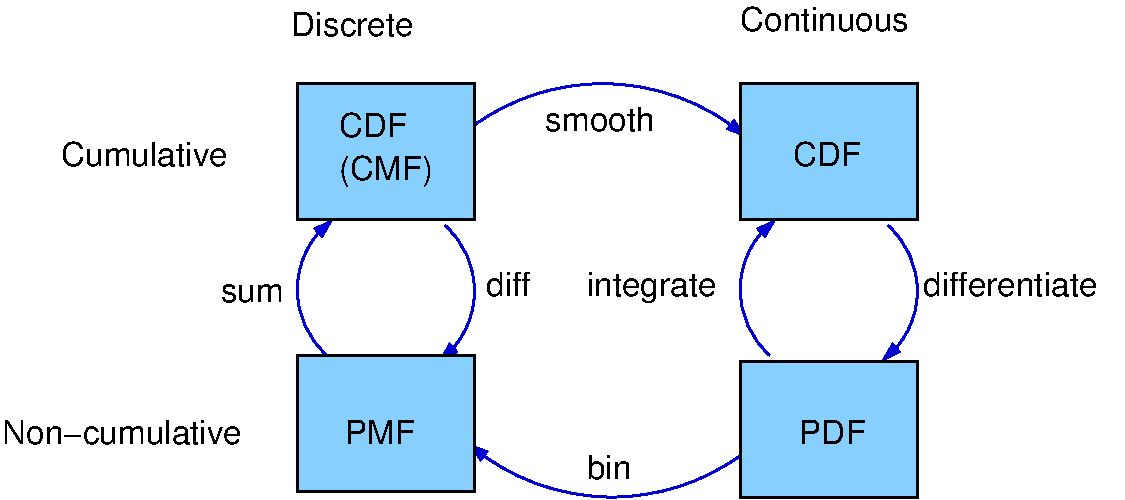
\includegraphics[height=2.2in]{figs/distribution_functions.pdf}}
\caption{A framework that relates representations of distribution
functions.}
\label{dist_framework}
\end{figure}

At this point we have seen PMFs, CDFs and PDFs; let's take a minute
to review.  Figure~\ref{dist_framework} shows how these functions relate
to each other.
\index{Pmf}
\index{Cdf}
\index{Pdf}

We started with PMFs, which represent the probabilities for a discrete
set of values.  To get from a PMF to a CDF, you add up the probability
masses to get cumulative probabilities.  
To get from a CDF back to a PMF, you compute differences in cumulative
probabilities.  We'll see the implementation of these operations
in the next few sections.
\index{cumulative probability}

A PDF is the derivative of a continuous CDF; or, equivalently,
a CDF is the integral of a PDF.  Remember that a PDF maps from
values to probability densities; to get a probability, you have to
integrate.
\index{discrete distribution}
\index{continuous distribution}
\index{smoothing}

To get from a discrete to a continuous distribution, you can perform
various kinds of smoothing.  One form of smoothing is to assume that
the data come from an analytic continuous distribution
(like exponential or normal) and to estimate the parameters of that
distribution.  Another option is kernel density estimation.
\index{exponential distribution}
\index{distribution!exponential}
\index{normal distribution}
\index{distribution!normal}
\index{Gaussian distribution}
\index{distribution!Gaussian}

The opposite of smoothing is {\bf discretizing}, or quantizing.  If you
evaluate a PDF at discrete points, you can generate a PMF that is an
approximation of the PDF.  You can get a better approximation using
numerical integration.  \index{discretize}
\index{quantize}
\index{binning}

To distinguish between continuous and discrete CDFs, it might be
better for a discrete CDF to be a ``cumulative mass function,'' but as
far as I can tell no one uses that term.  \index{CDF}



\section{Hist implementation}

At this point you should know how to use the basic types provided
by {\tt thinkstats2}: Hist, Pmf, Cdf, and Pdf.  The next few sections
provide details about how they are implemented.  This material
might help you use these classes more effectively, but it is not
strictly necessary.
\index{Hist}

Hist and Pmf inherit from a parent class called \verb"_DictWrapper".
The leading underscore indicates that this class is ``internal;'' that
is, it should not be used by code in other modules.  The name
indicates what it is: a dictionary wrapper.  Its primary attribute is
{\tt d}, the dictionary that maps from values to their frequencies.
\index{DictWrapper}
\index{internal class}
\index{wrapper}

The values can be any hashable type.  The frequencies should be integers,
but can be any numeric type.
\index{hashable}

\verb"_DictWrapper" contains methods appropriate for both
Hist and Pmf, including \verb"__init__", {\tt Values},
{\tt Items} and {\tt Render}.  It also provides modifier
methods {\tt Set}, {\tt Incr}, {\tt Mult}, and {\tt Remove}.  These
methods are all implemented with dictionary operations.  For example:
\index{dictionary}

\begin{verbatim}
# class _DictWrapper

    def Incr(self, x, term=1):
        self.d[x] = self.d.get(x, 0) + term

    def Mult(self, x, factor):
        self.d[x] = self.d.get(x, 0) * factor

    def Remove(self, x):
        del self.d[x]
\end{verbatim}

Hist also provides {\tt Freq}, which looks up the frequency
of a given value.
\index{frequency}

Because Hist operators and methods are based on dictionaries,
these methods are constant time operations;
that is, their run time does not increase as the Hist gets bigger.
\index{Hist}


\section{Pmf implementation}

Pmf and Hist are almost the same thing, except that a Pmf
maps values to floating-point probabilities, rather than integer
frequencies.  If the sum of the probabilities is 1, the Pmf is normalized.
\index{Pmf}

Pmf provides {\tt Normalize}, which computes the sum of the
probabilities and divides through by a factor:

\begin{verbatim}
# class Pmf

    def Normalize(self, fraction=1.0):
        total = self.Total()
        if total == 0.0:
            raise ValueError('Total probability is zero.')

        factor = float(fraction) / total
        for x in self.d:
            self.d[x] *= factor

        return total
\end{verbatim}

{\tt fraction} determines the sum of the probabilities after
normalizing; the default value is 1.  If the total probability is 0,
the Pmf cannot be normalized, so {\tt Normalize} raises {\tt
  ValueError}.

Hist and Pmf have the same constructor.  It can take
as an argument a {\tt dict}, Hist, Pmf or Cdf, a pandas
Series, a list of (value, frequency) pairs, or a sequence of values.
\index{Hist}

If you instantiate a Pmf, the result is normalized.  If you
instantiate a Hist, it is not.  To construct an unnormalized Pmf,
you can create an empty Pmf and modify it.  The Pmf modifiers do
not renormalize the Pmf.


\section{Cdf implementation}

A CDF maps from values to cumulative probabilities, so I could have
implemented Cdf as a \verb"_DictWrapper".  But the values in a CDF are
ordered and the values in a \verb"_DictWrapper" are not.  Also, it is
often useful to compute the inverse CDF; that is, the map from
cumulative probability to value.  So the implementaion I chose is two
sorted lists.  That way I can use binary search to do a forward or
inverse lookup in logarithmic time.
\index{Cdf}
\index{binary search}
\index{cumulative probability}
\index{DictWrapper}
\index{inverse CDF}
\index{CDF, inverse}

The Cdf constructor can take as a parameter a sequence of values
or a pandas Series, a dictionary that maps from values to
probabilities, a sequence of (value, probability) pairs, a Hist, Pmf,
or Cdf.  Or if it is given two parameters, it treats them as a sorted
sequence of values and the sequence of corresponding cumulative
probabilities.

Given a sequence, pandas Series, or dictionary, the constructor makes
a Hist.  Then it uses the Hist to initialize the attributes:

\begin{verbatim}
        self.xs, freqs = zip(*sorted(dw.Items()))
        self.ps = np.cumsum(freqs, dtype=np.float)
        self.ps /= self.ps[-1]
\end{verbatim}

{\tt xs} is the sorted list of values; {\tt freqs} is the list
of corresponding frequencies.  {\tt np.cumsum} computes
the cumulative sum of the frequencies.  Dividing through by the
total frequency yields cumulative probabilities.
For {\tt n} values, the time to construct the
Cdf is proportional to $n \log n$.
\index{frequency}

Here is the implementation of {\tt Prob}, which takes a value
and returns its cumulative probability: 

\begin{verbatim}
# class Cdf
    def Prob(self, x):
        if x < self.xs[0]:
            return 0.0
        index = bisect.bisect(self.xs, x)
        p = self.ps[index - 1]
        return p
\end{verbatim}

The {\tt bisect} module provides an implementation of binary search.
And here is the implementation of {\tt Value}, which takes a
cumulative probability and returns the corresponding value:

\begin{verbatim}
# class Cdf
    def Value(self, p):
        if p < 0 or p > 1:
            raise ValueError('p must be in range [0, 1]')

        index = bisect.bisect_left(self.ps, p)
        return self.xs[index]
\end{verbatim}

Given a Cdf, we can compute the Pmf by computing differences between
consecutive cumulative probabilities.  If you call the Cdf constructor
and pass a Pmf, it computes differences by calling {\tt Cdf.Items}:
\index{Pmf}
\index{Cdf}

\begin{verbatim}
# class Cdf
    def Items(self):
        a = self.ps
        b = np.roll(a, 1)
        b[0] = 0
        return zip(self.xs, a-b)
\end{verbatim}

{\tt np.roll} shifts the elements of {\tt a} to the right, and ``rolls''
the last one back to the beginning.  We replace the first element of
{\tt b} with 0 and then compute the difference {\tt a-b}.  The result
is a NumPy array of probabilities.
\index{NumPy}

Cdf provides {\tt Shift} and {\tt Scale}, which modify the
values in the Cdf, but the probabilities should be treated as
immutable.


\section{Moments}
\index{moment}

Any time you take a sample and reduce it to a single number, that
number is a statistic.  The statistics we have seen so far include
mean, variance, median, and interquartile range.

A {\bf raw moment} is a kind of statistic.  If you have a sample of
values, $x_i$, the $k$th raw moment is:
%
\[ m'_k = \frac{1}{n} \sum_i x_i^k \]
%
Or if you prefer Python notation:

\begin{verbatim}
def RawMoment(xs, k):
    return sum(x**k for x in xs) / len(xs)
\end{verbatim}

When $k=1$ the result is the sample mean, $\xbar$.  The other
raw moments don't mean much by themselves, but they are used
in some computations.

The {\bf central moments} are more useful.  The
$k$th central moment is:
%
\[ m_k = \frac{1}{n} \sum_i (x_i - \xbar)^k \]
%
Or in Python:

\begin{verbatim}
def CentralMoment(xs, k):
    mean = RawMoment(xs, 1)
    return sum((x - mean)**k for x in xs) / len(xs)
\end{verbatim}

When $k=2$ the result is the second central moment, which you might
recognize as variance.  The definition of variance gives a hint about
why these statistics are called moments.  If we attach a weight along a
ruler at each location, $x_i$, and then spin the ruler around
the mean, the moment of inertia of the spinning weights is the variance
of the values.  If you are not familiar with moment of inertia, see
\url{http://en.wikipedia.org/wiki/Moment_of_inertia}.  \index{moment
  of inertia}

When you report moment-based statistics, it is important to think
about the units.  For example, if the values $x_i$ are in cm, the
first raw moment is also in cm.  But the second moment is in
cm$^2$, the third moment is in cm$^3$, and so on.

Because of these units, moments are hard to interpret by themselves.
That's why, for the second moment, it is common to report standard
deviation, which is the square root of variance, so it is in the same
units as $x_i$.
\index{standard deviation}


\section{Skewness}
\index{skewness}

{\bf Skewness} is a property that describes the shape of a distribution.
If the distribution is symmetric around its central tendency, it is
unskewed.  If the values extend farther to the right, it is ``right
skewed'' and if the values extend left, it is ``left skewed.''
\index{central tendency}

This use of ``skewed'' does not have the usual connotation of
``biased.''  Skewness only describes the shape of the distribution;
it says nothing about whether the sampling process might have been
biased.
\index{bias}
\index{sample skewness}

Several statistics are commonly used to quantify the skewness of a
distribution.  Given a sequence of values, $x_i$, the {\bf sample
  skewness}, $g_1$, can be computed like this:

\begin{verbatim}
def StandardizedMoment(xs, k):
    var = CentralMoment(xs, 2)
    std = math.sqrt(var)
    return CentralMoment(xs, k) / std**k

def Skewness(xs):
    return StandardizedMoment(xs, 3)
\end{verbatim}

$g_1$ is the third {\bf standardized moment}, which means that it has
been normalized so it has no units.
\index{standardized moment}

Negative skewness indicates that a distribution 
skews left; positive skewness indicates
that a distribution skews right.  The magnitude of $g_1$ indicates
the strength of the skewness, but by itself it is not easy to
interpret.

In practice, computing sample skewness is usually not
a good idea.  If there are any outliers, they
have a disproportionate effect on $g_1$.
\index{outlier}

Another way to evaluate the asymmetry of a distribution is to look
at the relationship between the mean and median.
Extreme values have more effect on the mean than the median, so
in a distribution that skews left, the mean is less than the median.
In a distribution that skews right, the mean is greater.
\index{symmetric}
\index{Pearson median skewness}

{\bf Pearson's median skewness coefficient} is a measure
of skewness based on the difference between the
sample mean and median:
%
\[ g_p = 3 (\xbar - m) / S \]
%
Where $\xbar$ is the sample mean, $m$ is the median, and
$S$ is the standard deviation.  Or in Python:
\index{standard deviation}

\begin{verbatim}
def Median(xs):
    cdf = thinkstats2.Cdf(xs)
    return cdf.Value(0.5)

def PearsonMedianSkewness(xs):
    median = Median(xs)
    mean = RawMoment(xs, 1)
    var = CentralMoment(xs, 2)
    std = math.sqrt(var)
    gp = 3 * (mean - median) / std
    return gp
\end{verbatim}

This statistic is {\bf robust}, which means that it is less vulnerable
to the effect of outliers.
\index{robust}
\index{outlier}

\begin{figure}
\centerline{\includegraphics[height=2.2in]{figs/density_totalwgt_kde.pdf}}
\caption{Estimated PDF of birthweight data from the NSFG.}
\label{density_totalwgt_kde}
\end{figure}

As an example, let's look at the skewness of birth weights in the
NSFG pregnancy data.  Here's the code to estimate and plot the PDF:
\index{thinkplot}

\begin{verbatim}
    live, firsts, others = first.MakeFrames()
    data = live.totalwgt_lb.dropna()
    pdf = thinkstats2.EstimatedPdf(data)
    thinkplot.Pdf(pdf, label='birth weight')
\end{verbatim}

Figure~\ref{density_totalwgt_kde} shows the result.  The left tail appears
longer than the right, so we suspect the distribution is skewed left.
The mean, 7.27 lbs, is a bit less than
the median, 7.38 lbs, so that is consistent with left skew.
And both skewness coefficients are negative:
sample skewness is -0.59;
Pearson's median skewness is -0.23.
\index{skewness}
\index{dropna}
\index{NaN}

\begin{figure}
\centerline{\includegraphics[height=2.2in]{figs/density_wtkg2_kde.pdf}}
\caption{Estimated PDF of adult weight data from the BRFSS.}
\label{density_wtkg2_kde}
\end{figure}

Now let's compare this distribution to the distribution of adult
weight in the BRFSS.  Again, here's the code:
\index{thinkplot}

\begin{verbatim}
    df = brfss.ReadBrfss(nrows=None)
    data = df.wtkg2.dropna()
    pdf = thinkstats2.EstimatedPdf(data)
    thinkplot.Pdf(pdf, label='adult weight')
\end{verbatim}

Figure~\ref{density_wtkg2_kde} shows the result.  The distribution
appears skewed to the right.  Sure enough, the mean, 79.0, is bigger
than the median, 77.3.  The sample skewness is 1.1 and Pearson's
median skewness is 0.26.
\index{dropna}
\index{NaN}

The sign of the skewness coefficient indicates whether the distribution
skews left or right, but other than that, they are hard to interpret.
Sample skewness is less robust; that is, it is more
susceptible to outliers.  As a result it is less reliable
when applied to skewed distributions, exactly when it would be most
relevant.
\index{outlier}
\index{robust}

Pearson's median skewness is based on a computed mean and variance,
so it is also susceptible to outliers, but since it does not depend
on a third moment, it is somewhat more robust.
\index{Pearson median skewness}


\section{Exercises}

A solution to this exercise is in \verb"chap06soln.py".

\begin{exercise}

The distribution of income is famously skewed to the right.  In this
exercise, we'll measure how strong that skew is.
\index{skewness}
\index{income}

The Current Population Survey (CPS) is a joint effort of the Bureau
of Labor Statistics and the Census Bureau to study income and related
variables.  Data collected in 2013 is available from
\url{http://www.census.gov/hhes/www/cpstables/032013/hhinc/toc.htm}.
I downloaded {\tt hinc06.xls}, which is an Excel spreadsheet with
information about household income, and converted it to {\tt hinc06.csv},
a CSV file you will find in the repository for this book.  You
will also find {\tt hinc2.py}, which reads this file and transforms
the data.
\index{Current Population Survey}
\index{Bureau of Labor Statistics}
\index{Census Bureau}

The dataset is in the form of a series of income ranges and the number
of respondents who fell in each range.  The lowest range includes
respondents who reported annual household income ``Under \$5000.''
The highest range includes respondents who made ``\$250,000 or
more.''

To estimate mean and other statistics from these data, we have to
make some assumptions about the lower and upper bounds, and how
the values are distributed in each range.  {\tt hinc2.py} provides
{\tt InterpolateSample}, which shows one way to model
this data.  It takes a DataFrame with a column, {\tt income}, that
contains the upper bound of each range, and {\tt freq}, which contains
the number of respondents in each frame.
\index{DataFrame}
\index{model}

It also takes \verb"log_upper", which is an assumed upper bound
on the highest range, expressed in {\tt log10} dollars.  
The default value, \verb"log_upper=6.0" represents the assumption
that the largest income among the respondents is
$10^6$, or one million dollars.

{\tt InterpolateSample} generates a pseudo-sample; that is, a sample
of household incomes that yields the same number of respondents
in each range as the actual data.  It assumes that incomes in
each range are equally spaced on a log10 scale.

Compute the median, mean, skewness and Pearson's skewness of the
resulting sample.  What fraction of households reports a taxable
income below the mean?  How do the results depend on the assumed
upper bound?
\end{exercise}


\section{Glossary}

\begin{itemize}

\item Probability density function (PDF): The derivative of a continuous CDF,
a function that maps a value to its probability density.
\index{PDF}
\index{probability density function}

\item Probability density: A quantity that can be integrated over a
  range of values to yield a probability.  If the values are in units
  of cm, for example, probability density is in units of probability
  per cm.
\index{probability density}

\item Kernel density estimation (KDE): An algorithm that estimates a PDF
based on a sample.
\index{kernel density estimation}
\index{KDE}

\item discretize: To approximate a continuous function or distribution
with a discrete function.  The opposite of smoothing.
\index{discretize}

\item raw moment: A statistic based on the sum of data raised to a power.
\index{raw moment}

\item central moment: A statistic based on deviation from the mean,
raised to a power.
\index{central moment}

\item standardized moment: A ratio of moments that has no units.
\index{standardized moment}

\item skewness: A measure of how asymmetric a distribution is.
\index{skewness}

\item sample skewness: A moment-based statistic intended to quantify
the skewness of a distribution.
\index{sample skewness}

\item Pearson's median skewness coefficient: A statistic intended to
  quantify the skewness of a distribution based on the median, mean,
  and standard deviation.
  \index{Pearson median skewness}

\item robust: A statistic is robust if it is relatively immune to the
  effect of outliers.
\index{robust}

\end{itemize}

